\begin{figure*}
\begin{minipage}[t]{0.25\linewidth - 3pt}

\begin{subfigure}[t]{\linewidth}
\begin{minipage}[t]{\matrixscale\linewidth}
\resizebox{\linewidth}{!}{%
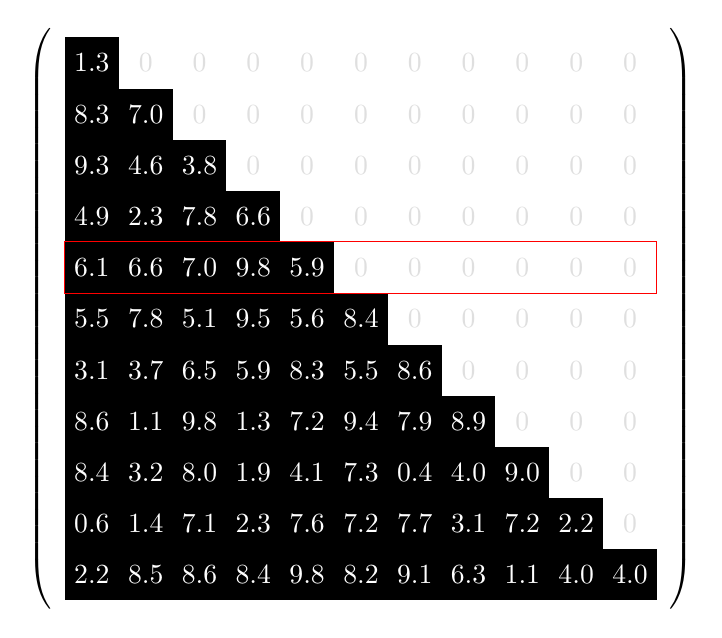
\begin{tikzpicture}[>=latex]
  \matrix (A) [matrix of math nodes,
              nodes = {whclsty},
              left delimiter  = (,
              right delimiter = ),
              ampersand replacement=\&] at (0,0)
  {
|[nzsty]|1.3 \& \zecl \& \zecl \& \zecl \& \zecl \& \zecl \& \zecl \& \zecl \& \zecl \& \zecl \& \zecl \\
|[nzsty]|8.3 \& |[nzsty]|7.0 \& \zecl \& \zecl \& \zecl \& \zecl \& \zecl \& \zecl \& \zecl \& \zecl \& \zecl \\
|[nzsty]|9.3 \& |[nzsty]|4.6 \& |[nzsty]|3.8 \& \zecl \& \zecl \& \zecl \& \zecl \& \zecl \& \zecl \& \zecl \& \zecl \\
|[nzsty]|4.9 \& |[nzsty]|2.3 \& |[nzsty]|7.8 \& |[nzsty]|6.6 \& \zecl \& \zecl \& \zecl \& \zecl \& \zecl \& \zecl \& \zecl \\
|[nzsty]|6.1 \& |[nzsty]|6.6 \& |[nzsty]|7.0 \& |[nzsty]|9.8 \& |[nzsty]|5.9 \& \zecl \& \zecl \& \zecl \& \zecl \& \zecl \& \zecl \\
|[nzsty]|5.5 \& |[nzsty]|7.8 \& |[nzsty]|5.1 \& |[nzsty]|9.5 \& |[nzsty]|5.6 \& |[nzsty]|8.4 \& \zecl \& \zecl \& \zecl \& \zecl \& \zecl \\
|[nzsty]|3.1 \& |[nzsty]|3.7 \& |[nzsty]|6.5 \& |[nzsty]|5.9 \& |[nzsty]|8.3 \& |[nzsty]|5.5 \& |[nzsty]|8.6 \& \zecl \& \zecl \& \zecl \& \zecl \\
|[nzsty]|8.6 \& |[nzsty]|1.1 \& |[nzsty]|9.8 \& |[nzsty]|1.3 \& |[nzsty]|7.2 \& |[nzsty]|9.4 \& |[nzsty]|7.9 \& |[nzsty]|8.9 \& \zecl \& \zecl \& \zecl \\
|[nzsty]|8.4 \& |[nzsty]|3.2 \& |[nzsty]|8.0 \& |[nzsty]|1.9 \& |[nzsty]|4.1 \& |[nzsty]|7.3 \& |[nzsty]|0.4 \& |[nzsty]|4.0 \& |[nzsty]|9.0 \& \zecl \& \zecl \\
|[nzsty]|0.6 \& |[nzsty]|1.4 \& |[nzsty]|7.1 \& |[nzsty]|2.3 \& |[nzsty]|7.6 \& |[nzsty]|7.2 \& |[nzsty]|7.7 \& |[nzsty]|3.1 \& |[nzsty]|7.2 \& |[nzsty]|2.2 \& \zecl \\
|[nzsty]|2.2 \& |[nzsty]|8.5 \& |[nzsty]|8.6 \& |[nzsty]|8.4 \& |[nzsty]|9.8 \& |[nzsty]|8.2 \& |[nzsty]|9.1 \& |[nzsty]|6.3 \& |[nzsty]|1.1 \& |[nzsty]|4.0 \& |[nzsty]|4.0 \\
  };

  \draw[hlsty] (A-5-1.south west) rectangle (A-5-11.north east);
\end{tikzpicture}%
}
\aftermatrix
\end{minipage}
\scalebox{\formatscale}{%
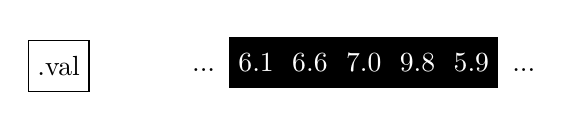
\begin{tikzpicture}[>=latex]
  \matrix (vals) [matrix of math nodes,
              nodes = {whclsty},
              ampersand replacement=\&,
              anchor=north west] at (0,0)
  {
... \& |[nzsty]|6.1 \& |[nzsty]|6.6 \& |[nzsty]|7.0 \& |[nzsty]|9.8 \& |[nzsty]|5.9 \& ... \\
  };

  \node [draw, whclsty, left=of vals] {\juliainline{.val}};

\end{tikzpicture}%
}
\afterformat
\resizebox{\linewidth}{!}{%
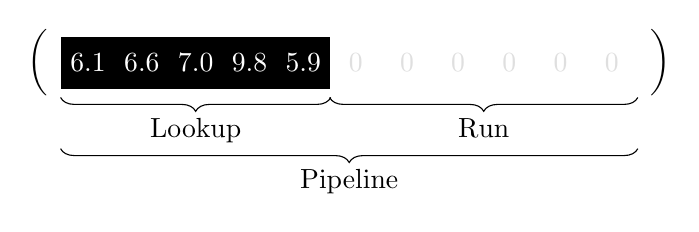
\begin{tikzpicture}[>=latex]
  \matrix (A) [matrix of math nodes,
              nodes = {whclsty},
              left delimiter  = (,
              right delimiter = ),
              ampersand replacement=\&] at (0,0)
  {
  |[nzsty]|6.1 \& |[nzsty]|6.6 \& |[nzsty]|7.0 \& |[nzsty]|9.8 \& |[nzsty]|5.9 \& \zecl \& \zecl \& \zecl \& \zecl \& \zecl \& \zecl \\
  };

  \draw[lpltsty] ([yshift=-0*\myunit]A-1-1.south west) -- ([yshift=-0*\myunit]A-1-5.south east) node[namesty]{Lookup};
  \draw[lpltsty] ([yshift=-0*\myunit]A-1-6.south west) -- ([yshift=-0*\myunit]A-1-11.south east) node[namesty]{Run};
  \draw[lpltsty] ([yshift=-1*\myunit]A-1-1.south west) -- ([yshift=-1*\myunit]A-1-11.south east) node[namesty]{Pipeline};
\end{tikzpicture}%
} 
\begin{juliacode}
offset = i*(i-1)/2
Pipeline(
  Phase(
    stride = i,
    body = Lookup(
      body(j) = val[offset+j])),
  Phase(
    body = Run(0)))
\end{juliacode}
\caption{Lower Triangular}\label{fig:structure:lotri}
\end{subfigure}
\beforematrix

\begin{subfigure}{\linewidth}
\begin{minipage}{\matrixscale\linewidth}
\documentclass{standalone}
\usepackage{tikz}
\usetikzlibrary{matrix,arrows,decorations.pathmorphing,decorations.pathreplacing,calc,positioning}
\usepackage{xcolor}
% all other packages and stuff you need for the picture
\newcommand{\myunit}{0.65 cm}
\newcommand{\myraise}{3pt}
\tikzset{
    lpltsty/.style={decorate, decoration = {brace,mirror,raise=3pt,amplitude=5pt}},
    namesty/.style={pos=0.5,below=7pt},
    scalarsty/.style={draw,fill=white,rectangle,minimum size=\myunit,anchor=center},
    indexsty/.style={fill,fill=white,rectangle,minimum width=\myunit,anchor=center},
    touchsty/.style={fill,fill=red,rectangle,minimum size=\myunit},
    ycsty/.style={fill,fill=yellow,rectangle,minimum size=\myunit},
    brcsty/.style={fill,fill=brown,rectangle,minimum size=\myunit},
    blcsty/.style={fill,fill=cyan!20,rectangle,minimum size=\myunit},
    becsty/.style={fill,fill=beige,rectangle,minimum size=\myunit},
    ocsty/.style={fill,fill=orange,rectangle,minimum size=\myunit},
    whclsty/.style={fill,fill=white,rectangle,minimum size=\myunit},
    zcsty/.style={fill,fill=white,rectangle,minimum size=\myunit,text=zerogray},
    nzsty/.style={fill,fill=black,rectangle,minimum size=\myunit,text=white},
    rcsty/.style={fill,fill=purple,rectangle,minimum size=\myunit},
    pcsty/.style={fill,fill=pink,rectangle,minimum size=\myunit},
    lcsty/.style={fill,fill=blue,rectangle,minimum size=\myunit},
    bcsty/.style={fill,fill=black,rectangle,minimum size=\myunit, text=white},
    hlsty/.style={draw=red},
}


\colorlet{zerogray}{gray!25}
\colorlet{beige}{brown!70}

\newcommand{\ylcl}{|[ycsty]|1}
\newcommand{\recl}{|[rcsty]|2}
\newcommand{\picl}{|[pcsty]|3}
\newcommand{\blcl}{|[blcsty]|1}
\newcommand{\brcl}{|[brcsty]|2}
\newcommand{\becl}{|[becsty]|3}
\newcommand{\orcl}{|[ocsty]|4}
\newcommand{\bkcl}{|[bcsty]|5}
\newcommand{\whcl}{|[whclsty]|0}
\newcommand{\zecl}{|[zcsty]|0}

\newcommand{\formatscale}{0.5}
\newcommand{\matrixscale}{0.69}
\begin{document}

\resizebox{\linewidth}{!}{%
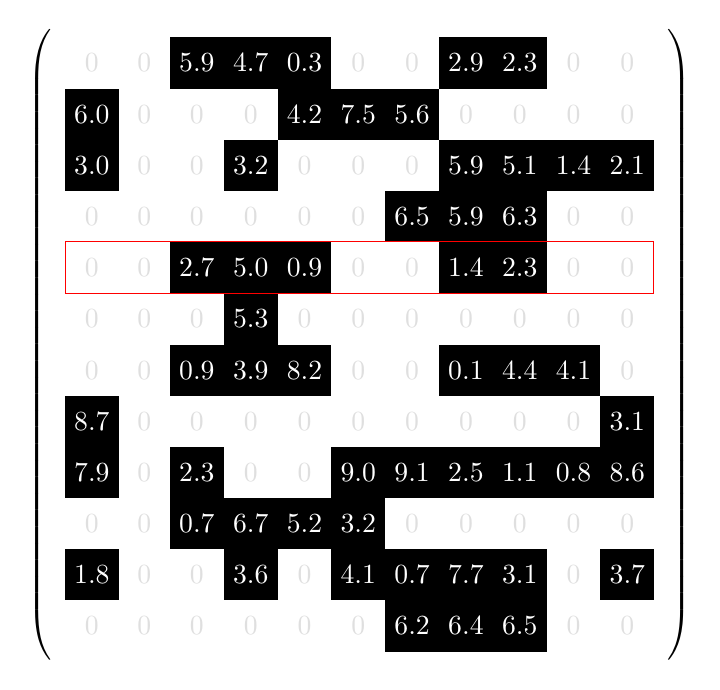
\begin{tikzpicture}[>=latex]
\matrix (A) [matrix of math nodes,
            nodes = {whclsty},
            left delimiter  = (,
            right delimiter = ),
            ampersand replacement=\&,
            anchor=north west] at (0,0)
{
  \zecl \& \zecl \& |[nzsty]|5.9 \& |[nzsty]|4.7 \& |[nzsty]|0.3 \& \zecl \& \zecl \& |[nzsty]|2.9 \& |[nzsty]|2.3 \& \zecl \& \zecl \\
  |[nzsty]|6.0 \& \zecl \& \zecl \& \zecl \& |[nzsty]|4.2 \& |[nzsty]|7.5 \& |[nzsty]|5.6 \& \zecl \& \zecl \& \zecl \& \zecl \\
  |[nzsty]|3.0 \& \zecl \& \zecl \& |[nzsty]|3.2 \& \zecl \& \zecl \& \zecl \& |[nzsty]|5.9 \& |[nzsty]|5.1 \& |[nzsty]|1.4 \& |[nzsty]|2.1 \\
  \zecl \& \zecl \& \zecl \& \zecl \& \zecl \& \zecl \& |[nzsty]|6.5 \& |[nzsty]|5.9 \& |[nzsty]|6.3 \& \zecl \& \zecl \\
  \zecl \& \zecl \& |[nzsty]|2.7 \& |[nzsty]|5.0 \& |[nzsty]|0.9 \& \zecl \& \zecl \& |[nzsty]|1.4 \& |[nzsty]|2.3 \& \zecl \& \zecl \\
  \zecl \& \zecl \& \zecl \& |[nzsty]|5.3 \& \zecl \& \zecl \& \zecl \& \zecl \& \zecl \& \zecl \& \zecl \\
  \zecl \& \zecl \& |[nzsty]|0.9 \& |[nzsty]|3.9 \& |[nzsty]|8.2 \& \zecl \& \zecl \& |[nzsty]|0.1 \& |[nzsty]|4.4 \& |[nzsty]|4.1 \& \zecl \\
  |[nzsty]|8.7 \& \zecl \& \zecl \& \zecl \& \zecl \& \zecl \& \zecl \& \zecl \& \zecl \& \zecl \& |[nzsty]|3.1 \\
  |[nzsty]|7.9 \& \zecl \& |[nzsty]|2.3 \& \zecl \& \zecl \& |[nzsty]|9.0 \& |[nzsty]|9.1 \& |[nzsty]|2.5 \& |[nzsty]|1.1 \& |[nzsty]|0.8 \& |[nzsty]|8.6 \\
  \zecl \& \zecl \& |[nzsty]|0.7 \& |[nzsty]|6.7 \& |[nzsty]|5.2 \& |[nzsty]|3.2 \& \zecl \& \zecl \& \zecl \& \zecl \& \zecl \\
  |[nzsty]|1.8 \& \zecl \& \zecl \& |[nzsty]|3.6 \& \zecl \& |[nzsty]|4.1 \& |[nzsty]|0.7 \& |[nzsty]|7.7 \& |[nzsty]|3.1 \& \zecl \& |[nzsty]|3.7 \\
  \zecl \& \zecl \& \zecl \& \zecl \& \zecl \& \zecl \& |[nzsty]|6.2 \& |[nzsty]|6.4 \& |[nzsty]|6.5 \& \zecl \& \zecl \\
};

\draw[hlsty] (A-5-1.south west) rectangle (A-5-11.north east);
\end{tikzpicture}}
\end{document}
\aftermatrix
\end{minipage}
\scalebox{\formatscale}{%
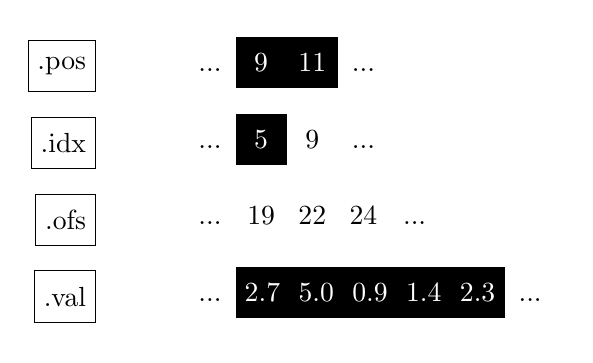
\begin{tikzpicture}[>=latex]
  \matrix (vals) [matrix of math nodes,
              nodes = {whclsty},
              ampersand replacement=\&,
              anchor=north west] at (0,0)
  {
  ... \& |[nzsty]|2.7 \& |[nzsty]|5.0 \& |[nzsty]|0.9 \& |[nzsty]|1.4 \& |[nzsty]|2.3 \& ... \\
  };
  \node [draw, whclsty, left=of vals] {\juliainline{.val}};

  \matrix (idx) [matrix of math nodes,
              nodes = {whclsty},
              ampersand replacement=\&,
              anchor=north west] at (0,3 * \myunit)
  {
  ... \& |[nzsty]|5 \& 9 \& ... \\
  };
  \node [draw, whclsty, left=of idx] {\juliainline{.idx}};

  \matrix (ofs) [matrix of math nodes,
              nodes = {whclsty},
              ampersand replacement=\&,
              anchor=north west] at (0,1.5 * \myunit)
  {
  ... \& 19 \& 22 \& 24 \& ... \\
  };
  \node [draw, whclsty, left=of ofs] {\juliainline{.ofs}};

  \matrix (pos) [matrix of math nodes,
              nodes = {whclsty},
              ampersand replacement=\&,
              anchor=north west] at (0,4.5 * \myunit)
  {
  ... \& |[nzsty]|9 \& |[nzsty]| 11 \& ... \\
  };
  \node [draw, whclsty, left=of pos] {\juliainline{.pos}};

\end{tikzpicture}%
}
\afterformat
\documentclass{standalone}
\usepackage{tikz}
\usetikzlibrary{matrix,arrows,decorations.pathmorphing,decorations.pathreplacing,calc,positioning}
\usepackage{xcolor}
% all other packages and stuff you need for the picture
\newcommand{\myunit}{0.65 cm}
\newcommand{\myraise}{3pt}
\tikzset{
    lpltsty/.style={decorate, decoration = {brace,mirror,raise=3pt,amplitude=5pt}},
    namesty/.style={pos=0.5,below=7pt},
    scalarsty/.style={draw,fill=white,rectangle,minimum size=\myunit,anchor=center},
    indexsty/.style={fill,fill=white,rectangle,minimum width=\myunit,anchor=center},
    touchsty/.style={fill,fill=red,rectangle,minimum size=\myunit},
    ycsty/.style={fill,fill=yellow,rectangle,minimum size=\myunit},
    brcsty/.style={fill,fill=brown,rectangle,minimum size=\myunit},
    blcsty/.style={fill,fill=cyan!20,rectangle,minimum size=\myunit},
    becsty/.style={fill,fill=beige,rectangle,minimum size=\myunit},
    ocsty/.style={fill,fill=orange,rectangle,minimum size=\myunit},
    whclsty/.style={fill,fill=white,rectangle,minimum size=\myunit},
    zcsty/.style={fill,fill=white,rectangle,minimum size=\myunit,text=zerogray},
    nzsty/.style={fill,fill=black,rectangle,minimum size=\myunit,text=white},
    rcsty/.style={fill,fill=purple,rectangle,minimum size=\myunit},
    pcsty/.style={fill,fill=pink,rectangle,minimum size=\myunit},
    lcsty/.style={fill,fill=blue,rectangle,minimum size=\myunit},
    bcsty/.style={fill,fill=black,rectangle,minimum size=\myunit, text=white},
    hlsty/.style={draw=red},
}


\colorlet{zerogray}{gray!25}
\colorlet{beige}{brown!70}

\newcommand{\ylcl}{|[ycsty]|1}
\newcommand{\recl}{|[rcsty]|2}
\newcommand{\picl}{|[pcsty]|3}
\newcommand{\blcl}{|[blcsty]|1}
\newcommand{\brcl}{|[brcsty]|2}
\newcommand{\becl}{|[becsty]|3}
\newcommand{\orcl}{|[ocsty]|4}
\newcommand{\bkcl}{|[bcsty]|5}
\newcommand{\whcl}{|[whclsty]|0}
\newcommand{\zecl}{|[zcsty]|0}

\newcommand{\formatscale}{0.5}
\newcommand{\matrixscale}{0.69}
\begin{document}

\resizebox{\linewidth}{!}{%
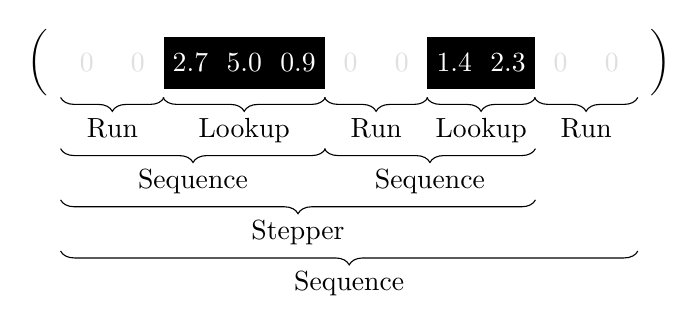
\begin{tikzpicture}[>=latex]
  \matrix (A) [matrix of math nodes,
              nodes = {whclsty},
              left delimiter  = (,
              right delimiter = ),
              ampersand replacement=\&] at (0,0)
  {
  \zecl \& \zecl \& |[nzsty]|2.7 \& |[nzsty]|5.0 \& |[nzsty]|0.9 \& \zecl \& \zecl \& |[nzsty]|1.4 \& |[nzsty]|2.3 \& \zecl \& \zecl \\
  };

  \draw[lpltsty] ([yshift=-0*\myunit]A-1-1.south west) -- ([yshift=-0*\myunit]A-1-2.south east) node[namesty]{Run};
  \draw[lpltsty] ([yshift=-0*\myunit]A-1-3.south west) -- ([yshift=-0*\myunit]A-1-5.south east) node[namesty]{Lookup};
  \draw[lpltsty] ([yshift=-0*\myunit]A-1-6.south west) -- ([yshift=-0*\myunit]A-1-7.south east) node[namesty]{Run};
  \draw[lpltsty] ([yshift=-0*\myunit]A-1-8.south west) -- ([yshift=-0*\myunit]A-1-9.south east) node[namesty]{Lookup};
  \draw[lpltsty] ([yshift=-0*\myunit]A-1-10.south west) -- ([yshift=-0*\myunit]A-1-11.south east) node[namesty]{Run};
  \draw[lpltsty] ([yshift=-1*\myunit]A-1-1.south west) -- ([yshift=-1*\myunit]A-1-5.south east) node[namesty]{Sequence};
  \draw[lpltsty] ([yshift=-1*\myunit]A-1-6.south west) -- ([yshift=-1*\myunit]A-1-9.south east) node[namesty]{Sequence};
  \draw[lpltsty] ([yshift=-2*\myunit]A-1-1.south west) -- ([yshift=-2*\myunit]A-1-9.south east) node[namesty]{Stepper};
  \draw[lpltsty] ([yshift=-3*\myunit]A-1-1.south west) -- ([yshift=-3*\myunit]A-1-11.south east) node[namesty]{Sequence};
\end{tikzpicture}%
}
\end{document}
\begin{juliacode}
Pipeline(
  Phase(
    stride = idx[pos[i+1]-1],
    body = begin
      p = pos[i]
      Stepper(
        seek(j) = (p = search(idx, j)),
        stride = idx[p],
        body = Pipeline(
          Phase(
            stride = idx[p]-(ofs[p+1]-ofs[p]),
            body = Run(0)),
          Phase(
            body = Lookup(
              body(j) =
                val[ofs[p+1]+j-idx[p]]))),
        next = p += 1))
  Phase(
    body = Run(0)))
\end{juliacode}
\caption{Clustered Matrix, VBL Format}\label{fig:structure:cluster-vbl}
\end{subfigure}

\end{minipage}\hspace{4pt}%
\begin{minipage}[t]{0.25\linewidth - 3pt}

\begin{subfigure}[t]{\linewidth}
\begin{minipage}[t]{\matrixscale\linewidth}
\documentclass{standalone}
\usepackage{tikz}
\usetikzlibrary{matrix,arrows,decorations.pathmorphing,decorations.pathreplacing,calc,positioning}
\usepackage{xcolor}
% all other packages and stuff you need for the picture
\newcommand{\myunit}{0.65 cm}
\newcommand{\myraise}{3pt}
\tikzset{
    lpltsty/.style={decorate, decoration = {brace,mirror,raise=3pt,amplitude=5pt}},
    namesty/.style={pos=0.5,below=7pt},
    scalarsty/.style={draw,fill=white,rectangle,minimum size=\myunit,anchor=center},
    indexsty/.style={fill,fill=white,rectangle,minimum width=\myunit,anchor=center},
    touchsty/.style={fill,fill=red,rectangle,minimum size=\myunit},
    ycsty/.style={fill,fill=yellow,rectangle,minimum size=\myunit},
    brcsty/.style={fill,fill=brown,rectangle,minimum size=\myunit},
    blcsty/.style={fill,fill=cyan!20,rectangle,minimum size=\myunit},
    becsty/.style={fill,fill=beige,rectangle,minimum size=\myunit},
    ocsty/.style={fill,fill=orange,rectangle,minimum size=\myunit},
    whclsty/.style={fill,fill=white,rectangle,minimum size=\myunit},
    zcsty/.style={fill,fill=white,rectangle,minimum size=\myunit,text=zerogray},
    nzsty/.style={fill,fill=black,rectangle,minimum size=\myunit,text=white},
    rcsty/.style={fill,fill=purple,rectangle,minimum size=\myunit},
    pcsty/.style={fill,fill=pink,rectangle,minimum size=\myunit},
    lcsty/.style={fill,fill=blue,rectangle,minimum size=\myunit},
    bcsty/.style={fill,fill=black,rectangle,minimum size=\myunit, text=white},
    hlsty/.style={draw=red},
}


\colorlet{zerogray}{gray!25}
\colorlet{beige}{brown!70}

\newcommand{\ylcl}{|[ycsty]|1}
\newcommand{\recl}{|[rcsty]|2}
\newcommand{\picl}{|[pcsty]|3}
\newcommand{\blcl}{|[blcsty]|1}
\newcommand{\brcl}{|[brcsty]|2}
\newcommand{\becl}{|[becsty]|3}
\newcommand{\orcl}{|[ocsty]|4}
\newcommand{\bkcl}{|[bcsty]|5}
\newcommand{\whcl}{|[whclsty]|0}
\newcommand{\zecl}{|[zcsty]|0}

\newcommand{\formatscale}{0.5}
\newcommand{\matrixscale}{0.69}
\begin{document}
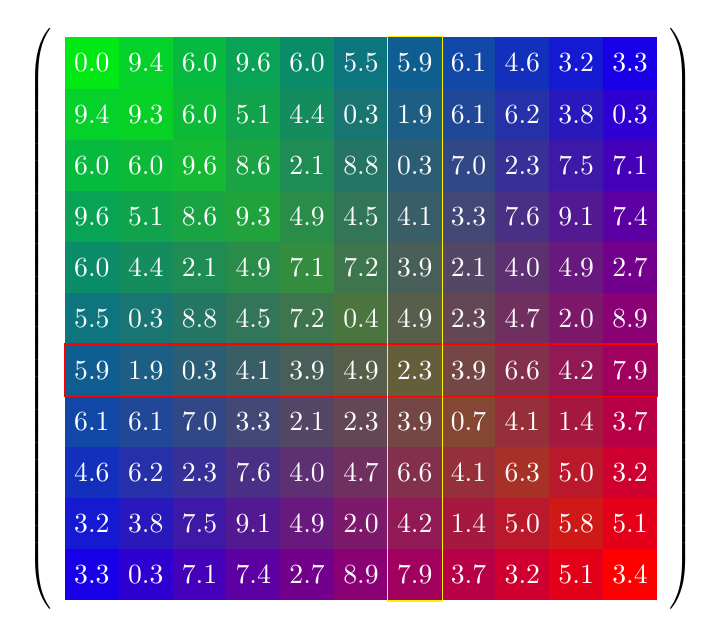
\begin{tikzpicture}[>=latex]
\matrix (A) [matrix of math nodes,
  nodes = {whclsty},
  left delimiter  = (,
  right delimiter = ),
  ampersand replacement=\&] at (0,0)
{
|[nzsty, fill=red!9!blue!9!green]|0.0 \& |[nzsty, fill=red!9!blue!18!green]|9.4 \& |[nzsty, fill=red!9!blue!27!green]|6.0 \& |[nzsty, fill=red!9!blue!36!green]|9.6 \& |[nzsty, fill=red!9!blue!45!green]|6.0 \& |[nzsty, fill=red!9!blue!54!green]|5.5 \& |[nzsty, fill=red!9!blue!63!green]|5.9 \& |[nzsty, fill=red!9!blue!72!green]|6.1 \& |[nzsty, fill=red!9!blue!81!green]|4.6 \& |[nzsty, fill=red!9!blue!90!green]|3.2 \& |[nzsty, fill=red!9!blue!100!green]|3.3 \\
|[nzsty, fill=red!9!blue!18!green]|9.4 \& |[nzsty, fill=red!18!blue!18!green]|9.3 \& |[nzsty, fill=red!18!blue!27!green]|6.0 \& |[nzsty, fill=red!18!blue!36!green]|5.1 \& |[nzsty, fill=red!18!blue!45!green]|4.4 \& |[nzsty, fill=red!18!blue!54!green]|0.3 \& |[nzsty, fill=red!18!blue!63!green]|1.9 \& |[nzsty, fill=red!18!blue!72!green]|6.1 \& |[nzsty, fill=red!18!blue!81!green]|6.2 \& |[nzsty, fill=red!18!blue!90!green]|3.8 \& |[nzsty, fill=red!18!blue!100!green]|0.3 \\
|[nzsty, fill=red!9!blue!27!green]|6.0 \& |[nzsty, fill=red!18!blue!27!green]|6.0 \& |[nzsty, fill=red!27!blue!27!green]|9.6 \& |[nzsty, fill=red!27!blue!36!green]|8.6 \& |[nzsty, fill=red!27!blue!45!green]|2.1 \& |[nzsty, fill=red!27!blue!54!green]|8.8 \& |[nzsty, fill=red!27!blue!63!green]|0.3 \& |[nzsty, fill=red!27!blue!72!green]|7.0 \& |[nzsty, fill=red!27!blue!81!green]|2.3 \& |[nzsty, fill=red!27!blue!90!green]|7.5 \& |[nzsty, fill=red!27!blue!100!green]|7.1 \\
|[nzsty, fill=red!9!blue!36!green]|9.6 \& |[nzsty, fill=red!18!blue!36!green]|5.1 \& |[nzsty, fill=red!27!blue!36!green]|8.6 \& |[nzsty, fill=red!36!blue!36!green]|9.3 \& |[nzsty, fill=red!36!blue!45!green]|4.9 \& |[nzsty, fill=red!36!blue!54!green]|4.5 \& |[nzsty, fill=red!36!blue!63!green]|4.1 \& |[nzsty, fill=red!36!blue!72!green]|3.3 \& |[nzsty, fill=red!36!blue!81!green]|7.6 \& |[nzsty, fill=red!36!blue!90!green]|9.1 \& |[nzsty, fill=red!36!blue!100!green]|7.4 \\
|[nzsty, fill=red!9!blue!45!green]|6.0 \& |[nzsty, fill=red!18!blue!45!green]|4.4 \& |[nzsty, fill=red!27!blue!45!green]|2.1 \& |[nzsty, fill=red!36!blue!45!green]|4.9 \& |[nzsty, fill=red!45!blue!45!green]|7.1 \& |[nzsty, fill=red!45!blue!54!green]|7.2 \& |[nzsty, fill=red!45!blue!63!green]|3.9 \& |[nzsty, fill=red!45!blue!72!green]|2.1 \& |[nzsty, fill=red!45!blue!81!green]|4.0 \& |[nzsty, fill=red!45!blue!90!green]|4.9 \& |[nzsty, fill=red!45!blue!100!green]|2.7 \\
|[nzsty, fill=red!9!blue!54!green]|5.5 \& |[nzsty, fill=red!18!blue!54!green]|0.3 \& |[nzsty, fill=red!27!blue!54!green]|8.8 \& |[nzsty, fill=red!36!blue!54!green]|4.5 \& |[nzsty, fill=red!45!blue!54!green]|7.2 \& |[nzsty, fill=red!54!blue!54!green]|0.4 \& |[nzsty, fill=red!54!blue!63!green]|4.9 \& |[nzsty, fill=red!54!blue!72!green]|2.3 \& |[nzsty, fill=red!54!blue!81!green]|4.7 \& |[nzsty, fill=red!54!blue!90!green]|2.0 \& |[nzsty, fill=red!54!blue!100!green]|8.9 \\
|[nzsty, fill=red!9!blue!63!green]|5.9 \& |[nzsty, fill=red!18!blue!63!green]|1.9 \& |[nzsty, fill=red!27!blue!63!green]|0.3 \& |[nzsty, fill=red!36!blue!63!green]|4.1 \& |[nzsty, fill=red!45!blue!63!green]|3.9 \& |[nzsty, fill=red!54!blue!63!green]|4.9 \& |[nzsty, fill=red!63!blue!63!green]|2.3 \& |[nzsty, fill=red!63!blue!72!green]|3.9 \& |[nzsty, fill=red!63!blue!81!green]|6.6 \& |[nzsty, fill=red!63!blue!90!green]|4.2 \& |[nzsty, fill=red!63!blue!100!green]|7.9 \\
|[nzsty, fill=red!9!blue!72!green]|6.1 \& |[nzsty, fill=red!18!blue!72!green]|6.1 \& |[nzsty, fill=red!27!blue!72!green]|7.0 \& |[nzsty, fill=red!36!blue!72!green]|3.3 \& |[nzsty, fill=red!45!blue!72!green]|2.1 \& |[nzsty, fill=red!54!blue!72!green]|2.3 \& |[nzsty, fill=red!63!blue!72!green]|3.9 \& |[nzsty, fill=red!72!blue!72!green]|0.7 \& |[nzsty, fill=red!72!blue!81!green]|4.1 \& |[nzsty, fill=red!72!blue!90!green]|1.4 \& |[nzsty, fill=red!72!blue!100!green]|3.7 \\
|[nzsty, fill=red!9!blue!81!green]|4.6 \& |[nzsty, fill=red!18!blue!81!green]|6.2 \& |[nzsty, fill=red!27!blue!81!green]|2.3 \& |[nzsty, fill=red!36!blue!81!green]|7.6 \& |[nzsty, fill=red!45!blue!81!green]|4.0 \& |[nzsty, fill=red!54!blue!81!green]|4.7 \& |[nzsty, fill=red!63!blue!81!green]|6.6 \& |[nzsty, fill=red!72!blue!81!green]|4.1 \& |[nzsty, fill=red!81!blue!81!green]|6.3 \& |[nzsty, fill=red!81!blue!90!green]|5.0 \& |[nzsty, fill=red!81!blue!100!green]|3.2 \\
|[nzsty, fill=red!9!blue!90!green]|3.2 \& |[nzsty, fill=red!18!blue!90!green]|3.8 \& |[nzsty, fill=red!27!blue!90!green]|7.5 \& |[nzsty, fill=red!36!blue!90!green]|9.1 \& |[nzsty, fill=red!45!blue!90!green]|4.9 \& |[nzsty, fill=red!54!blue!90!green]|2.0 \& |[nzsty, fill=red!63!blue!90!green]|4.2 \& |[nzsty, fill=red!72!blue!90!green]|1.4 \& |[nzsty, fill=red!81!blue!90!green]|5.0 \& |[nzsty, fill=red!90!blue!90!green]|5.8 \& |[nzsty, fill=red!90!blue!100!green]|5.1 \\
|[nzsty, fill=red!9!blue!100!green]|3.3 \& |[nzsty, fill=red!18!blue!100!green]|0.3 \& |[nzsty, fill=red!27!blue!100!green]|7.1 \& |[nzsty, fill=red!36!blue!100!green]|7.4 \& |[nzsty, fill=red!45!blue!100!green]|2.7 \& |[nzsty, fill=red!54!blue!100!green]|8.9 \& |[nzsty, fill=red!63!blue!100!green]|7.9 \& |[nzsty, fill=red!72!blue!100!green]|3.7 \& |[nzsty, fill=red!81!blue!100!green]|3.2 \& |[nzsty, fill=red!90!blue!100!green]|5.1 \& |[nzsty, fill=red!100!blue!100!green]|3.4 \\
};

\draw[hlsty] (A-7-1.south west) rectangle (A-7-11.north east);
\draw[hlsty,color=yellow] (A-1-7.north east) rectangle (A-11-7.south west);
\end{tikzpicture}
\end{document}
\aftermatrix
\end{minipage}
\scalebox{\formatscale}{%
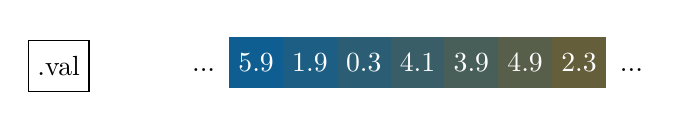
\begin{tikzpicture}[>=latex]
  \matrix (vals) [matrix of math nodes,
              nodes = {whclsty},
              ampersand replacement=\&,
              anchor=north west] at (0,0)
  {
  ... \& |[nzsty, fill=red!9!blue!63!green]|5.9 \& |[nzsty, fill=red!18!blue!63!green]|1.9 \& |[nzsty, fill=red!27!blue!63!green]|0.3 \& |[nzsty, fill=red!36!blue!63!green]|4.1 \& |[nzsty, fill=red!45!blue!63!green]|3.9 \& |[nzsty, fill=red!54!blue!63!green]|4.9 \& |[nzsty, fill=red!63!blue!63!green]|2.3 \& ... \\
  };
  \node [draw, whclsty, left=of vals] {\juliainline{.val}};

%  \matrix (size) [matrix of math nodes,
%  nodes = {whclsty},
%  ampersand replacement=\&,
%  anchor = north west] at (0,4.5*\myunit)
%  {
%  |[nzsty]|11\\
%  };
%  \node [draw, whclsty, left=of size] {\juliainline{.size}};

\end{tikzpicture}%
}
\afterformat
\resizebox{\linewidth}{!}{%
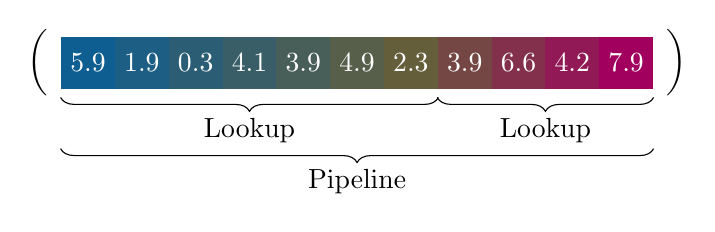
\begin{tikzpicture}[>=latex]
  \matrix (A) [matrix of math nodes,
              nodes = {whclsty},
              left delimiter  = (,
              right delimiter = ),
              ampersand replacement=\&] at (0,0)
  {
  |[nzsty, fill=red!9!blue!63!green]|5.9 \& |[nzsty, fill=red!18!blue!63!green]|1.9 \& |[nzsty, fill=red!27!blue!63!green]|0.3 \& |[nzsty, fill=red!36!blue!63!green]|4.1 \& |[nzsty, fill=red!45!blue!63!green]|3.9 \& |[nzsty, fill=red!54!blue!63!green]|4.9 \& |[nzsty, fill=red!63!blue!63!green]|2.3 \& |[nzsty, fill=red!63!blue!72!green]|3.9 \& |[nzsty, fill=red!63!blue!81!green]|6.6 \& |[nzsty, fill=red!63!blue!90!green]|4.2 \& |[nzsty, fill=red!63!blue!100!green]|7.9 \\
  };

  \draw[lpltsty] ([yshift=-0*\myunit]A-1-1.south west) -- ([yshift=-0*\myunit]A-1-7.south east) node[namesty]{Lookup};
  \draw[lpltsty] ([yshift=-0*\myunit]A-1-8.south west) -- ([yshift=-0*\myunit]A-1-11.south east) node[namesty]{Lookup};
  \draw[lpltsty] ([yshift=-1*\myunit]A-1-1.south west) -- ([yshift=-1*\myunit]A-1-11.south east) node[namesty]{Pipeline};
\end{tikzpicture}%
}  

\begin{juliacode}
offset = i*(i-1)/2
Pipeline(
  Phase(
    stride = i,
    body = Lookup(
      body(j) = val[offset+j])),
  Phase(
    body = Lookup(
      body(j) = val[j*(j-1)/2+i])))
\end{juliacode}
\caption{Symmetric}\label{fig:structure:sym}
\end{subfigure}
\beforematrix


\begin{subfigure}{\linewidth}
\begin{minipage}{\matrixscale\linewidth}
\documentclass{standalone}
\usepackage{tikz}
\usetikzlibrary{matrix,arrows,decorations.pathmorphing,decorations.pathreplacing,calc,positioning}
\usepackage{xcolor}
% all other packages and stuff you need for the picture
\newcommand{\myunit}{0.65 cm}
\newcommand{\myraise}{3pt}
\tikzset{
    lpltsty/.style={decorate, decoration = {brace,mirror,raise=3pt,amplitude=5pt}},
    namesty/.style={pos=0.5,below=7pt},
    scalarsty/.style={draw,fill=white,rectangle,minimum size=\myunit,anchor=center},
    indexsty/.style={fill,fill=white,rectangle,minimum width=\myunit,anchor=center},
    touchsty/.style={fill,fill=red,rectangle,minimum size=\myunit},
    ycsty/.style={fill,fill=yellow,rectangle,minimum size=\myunit},
    brcsty/.style={fill,fill=brown,rectangle,minimum size=\myunit},
    blcsty/.style={fill,fill=cyan!20,rectangle,minimum size=\myunit},
    becsty/.style={fill,fill=beige,rectangle,minimum size=\myunit},
    ocsty/.style={fill,fill=orange,rectangle,minimum size=\myunit},
    whclsty/.style={fill,fill=white,rectangle,minimum size=\myunit},
    zcsty/.style={fill,fill=white,rectangle,minimum size=\myunit,text=zerogray},
    nzsty/.style={fill,fill=black,rectangle,minimum size=\myunit,text=white},
    rcsty/.style={fill,fill=purple,rectangle,minimum size=\myunit},
    pcsty/.style={fill,fill=pink,rectangle,minimum size=\myunit},
    lcsty/.style={fill,fill=blue,rectangle,minimum size=\myunit},
    bcsty/.style={fill,fill=black,rectangle,minimum size=\myunit, text=white},
    hlsty/.style={draw=red},
}


\colorlet{zerogray}{gray!25}
\colorlet{beige}{brown!70}

\newcommand{\ylcl}{|[ycsty]|1}
\newcommand{\recl}{|[rcsty]|2}
\newcommand{\picl}{|[pcsty]|3}
\newcommand{\blcl}{|[blcsty]|1}
\newcommand{\brcl}{|[brcsty]|2}
\newcommand{\becl}{|[becsty]|3}
\newcommand{\orcl}{|[ocsty]|4}
\newcommand{\bkcl}{|[bcsty]|5}
\newcommand{\whcl}{|[whclsty]|0}
\newcommand{\zecl}{|[zcsty]|0}

\newcommand{\formatscale}{0.5}
\newcommand{\matrixscale}{0.69}
\begin{document}

\resizebox{\linewidth}{!}{%
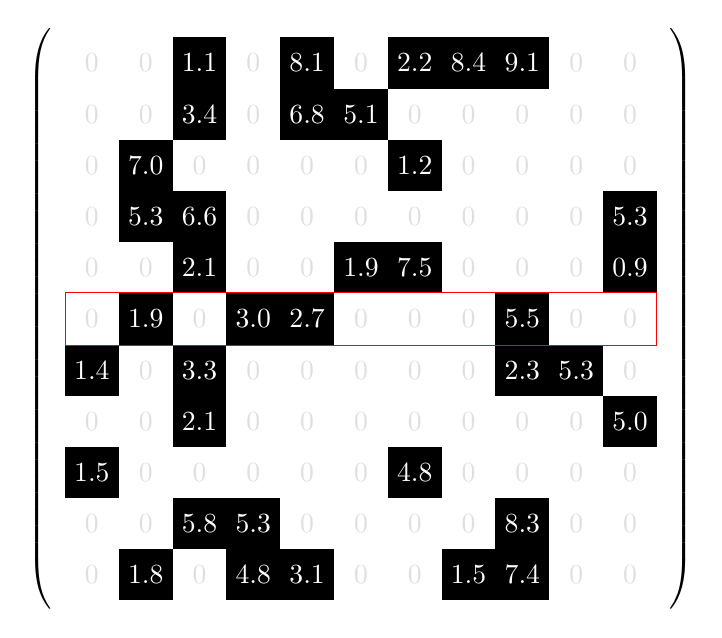
\begin{tikzpicture}[>=latex]
\matrix (A) [matrix of math nodes,
  nodes = {whclsty},
  left delimiter  = (,
  right delimiter = ),
  ampersand replacement=\&] at (0,0)
{
\zecl \& \zecl \& |[nzsty]|1.1 \& \zecl \& |[nzsty]|8.1 \& \zecl \& |[nzsty]|2.2 \& |[nzsty]|8.4 \& |[nzsty]|9.1 \& \zecl \& \zecl \\
\zecl \& \zecl \& |[nzsty]|3.4 \& \zecl \& |[nzsty]|6.8 \& |[nzsty]|5.1 \& \zecl \& \zecl \& \zecl \& \zecl \& \zecl \\
\zecl \& |[nzsty]|7.0 \& \zecl \& \zecl \& \zecl \& \zecl \& |[nzsty]|1.2 \& \zecl \& \zecl \& \zecl \& \zecl \\
\zecl \& |[nzsty]|5.3 \& |[nzsty]|6.6 \& \zecl \& \zecl \& \zecl \& \zecl \& \zecl \& \zecl \& \zecl \& |[nzsty]|5.3 \\
\zecl \& \zecl \& |[nzsty]|2.1 \& \zecl \& \zecl \& |[nzsty]|1.9 \& |[nzsty]|7.5 \& \zecl \& \zecl \& \zecl \& |[nzsty]|0.9 \\
\zecl \& |[nzsty]|1.9 \& \zecl \& |[nzsty]|3.0 \& |[nzsty]|2.7 \& \zecl \& \zecl \& \zecl \& |[nzsty]|5.5 \& \zecl \& \zecl \\
|[nzsty]|1.4 \& \zecl \& |[nzsty]|3.3 \& \zecl \& \zecl \& \zecl \& \zecl \& \zecl \& |[nzsty]|2.3 \& |[nzsty]|5.3 \& \zecl \\
\zecl \& \zecl \& |[nzsty]|2.1 \& \zecl \& \zecl \& \zecl \& \zecl \& \zecl \& \zecl \& \zecl \& |[nzsty]|5.0 \\
|[nzsty]|1.5 \& \zecl \& \zecl \& \zecl \& \zecl \& \zecl \& |[nzsty]|4.8 \& \zecl \& \zecl \& \zecl \& \zecl \\
\zecl \& \zecl \& |[nzsty]|5.8 \& |[nzsty]|5.3 \& \zecl \& \zecl \& \zecl \& \zecl \& |[nzsty]|8.3 \& \zecl \& \zecl \\
\zecl \& |[nzsty]|1.8 \& \zecl \& |[nzsty]|4.8 \& |[nzsty]|3.1 \& \zecl \& \zecl \& |[nzsty]|1.5 \& |[nzsty]|7.4 \& \zecl \& \zecl \\
};

\draw[hlsty] (A-6-1.south west) rectangle (A-6-11.north east);
\end{tikzpicture}%
}
\end{document}
\aftermatrix
\end{minipage}
\scalebox{\formatscale}{%
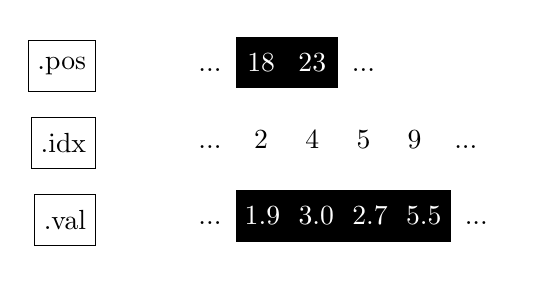
\begin{tikzpicture}[>=latex]
  \matrix (vals) [matrix of math nodes,
              nodes = {whclsty},
              ampersand replacement=\&,
              anchor=north west] at (0,0)
  {
  ... \& |[nzsty]|1.9 \& |[nzsty]|3.0 \& |[nzsty]|2.7 \& |[nzsty]|5.5 \& ... \\
  };
  \node [draw, whclsty, left=of vals] {\juliainline{.val}};

  \matrix (idx) [matrix of math nodes,
              nodes = {whclsty},
              ampersand replacement=\&,
              anchor=north west] at (0,1.5 * \myunit)
  {
  ... \& 2 \& 4 \& 5 \& 9 \& ... \\
  };
  \node [draw, whclsty, left=of idx] {\juliainline{.idx}};

  \matrix (pos) [matrix of math nodes,
              nodes = {whclsty},
              ampersand replacement=\&,
              anchor=north west] at (0,3 * \myunit)
  {
  ... \& |[nzsty]|18 \& |[nzsty]| 23 \& ... \\
  };
  \node [draw, whclsty, left=of pos] {\juliainline{.pos}};

\end{tikzpicture}%
}
\afterformat
\documentclass{standalone}
\usepackage{tikz}
\usetikzlibrary{matrix,arrows,decorations.pathmorphing,decorations.pathreplacing,calc,positioning}
\usepackage{xcolor}
% all other packages and stuff you need for the picture
\newcommand{\myunit}{0.65 cm}
\newcommand{\myraise}{3pt}
\tikzset{
    lpltsty/.style={decorate, decoration = {brace,mirror,raise=3pt,amplitude=5pt}},
    namesty/.style={pos=0.5,below=7pt},
    scalarsty/.style={draw,fill=white,rectangle,minimum size=\myunit,anchor=center},
    indexsty/.style={fill,fill=white,rectangle,minimum width=\myunit,anchor=center},
    touchsty/.style={fill,fill=red,rectangle,minimum size=\myunit},
    ycsty/.style={fill,fill=yellow,rectangle,minimum size=\myunit},
    brcsty/.style={fill,fill=brown,rectangle,minimum size=\myunit},
    blcsty/.style={fill,fill=cyan!20,rectangle,minimum size=\myunit},
    becsty/.style={fill,fill=beige,rectangle,minimum size=\myunit},
    ocsty/.style={fill,fill=orange,rectangle,minimum size=\myunit},
    whclsty/.style={fill,fill=white,rectangle,minimum size=\myunit},
    zcsty/.style={fill,fill=white,rectangle,minimum size=\myunit,text=zerogray},
    nzsty/.style={fill,fill=black,rectangle,minimum size=\myunit,text=white},
    rcsty/.style={fill,fill=purple,rectangle,minimum size=\myunit},
    pcsty/.style={fill,fill=pink,rectangle,minimum size=\myunit},
    lcsty/.style={fill,fill=blue,rectangle,minimum size=\myunit},
    bcsty/.style={fill,fill=black,rectangle,minimum size=\myunit, text=white},
    hlsty/.style={draw=red},
}


\colorlet{zerogray}{gray!25}
\colorlet{beige}{brown!70}

\newcommand{\ylcl}{|[ycsty]|1}
\newcommand{\recl}{|[rcsty]|2}
\newcommand{\picl}{|[pcsty]|3}
\newcommand{\blcl}{|[blcsty]|1}
\newcommand{\brcl}{|[brcsty]|2}
\newcommand{\becl}{|[becsty]|3}
\newcommand{\orcl}{|[ocsty]|4}
\newcommand{\bkcl}{|[bcsty]|5}
\newcommand{\whcl}{|[whclsty]|0}
\newcommand{\zecl}{|[zcsty]|0}

\newcommand{\formatscale}{0.5}
\newcommand{\matrixscale}{0.69}
\begin{document}

\resizebox{\linewidth}{!}{%
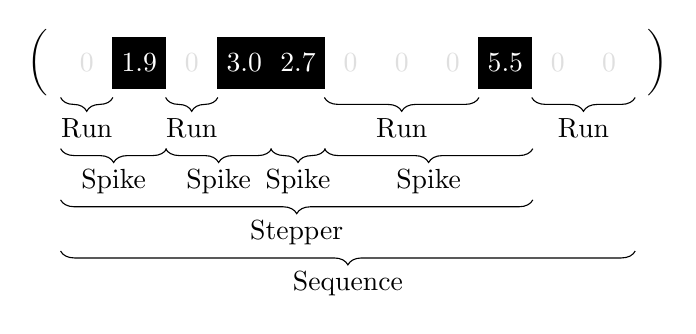
\begin{tikzpicture}[>=latex]
\matrix (A) [matrix of math nodes,
  nodes = {whclsty},
  left delimiter  = (,
  right delimiter = ),
  ampersand replacement=\&] at (0,0)
{
  \zecl \& |[nzsty]|1.9 \& \zecl \& |[nzsty]|3.0 \& |[nzsty]|2.7 \& \zecl \& \zecl \& \zecl \& |[nzsty]|5.5 \& \zecl \& \zecl \\
};

\draw[lpltsty] ([yshift=-0*\myunit]A-1-1.south west) -- ([yshift=-0*\myunit]A-1-1.south east) node[namesty]{Run};
%\draw[lpltsty] ([yshift=-0*\myunit]A-1-2.south west) -- ([yshift=-0*\myunit]A-1-2.south east) node[namesty]{Lookup};
\draw[lpltsty] ([yshift=-0*\myunit]A-1-3.south west) -- ([yshift=-0*\myunit]A-1-3.south east) node[namesty]{Run};
%\draw[lpltsty] ([yshift=-0*\myunit]A-1-4.south west) -- ([yshift=-0*\myunit]A-1-4.south east) node[namesty]{Lookup};
%\draw[lpltsty] ([yshift=-0*\myunit]A-1-5.south west) -- ([yshift=-0*\myunit]A-1-5.south east) node[namesty]{Lookup};
\draw[lpltsty] ([yshift=-0*\myunit]A-1-6.south west) -- ([yshift=-0*\myunit]A-1-8.south east) node[namesty]{Run};
%\draw[lpltsty] ([yshift=-0*\myunit]A-1-9.south west) -- ([yshift=-0*\myunit]A-1-9.south east) node[namesty]{Lookup};
\draw[lpltsty] ([yshift=-0*\myunit]A-1-10.south west) -- ([yshift=-0*\myunit]A-1-11.south east) node[namesty]{Run};

\draw[lpltsty] ([yshift=-1*\myunit]A-1-1.south west) -- ([yshift=-1*\myunit]A-1-2.south east) node[namesty]{Spike};
\draw[lpltsty] ([yshift=-1*\myunit]A-1-3.south west) -- ([yshift=-1*\myunit]A-1-4.south east) node[namesty]{Spike};
\draw[lpltsty] ([yshift=-1*\myunit]A-1-5.south west) -- ([yshift=-1*\myunit]A-1-5.south east) node[namesty]{Spike};
\draw[lpltsty] ([yshift=-1*\myunit]A-1-6.south west) -- ([yshift=-1*\myunit]A-1-9.south east) node[namesty]{Spike};

\draw[lpltsty] ([yshift=-2*\myunit]A-1-1.south west) -- ([yshift=-2*\myunit]A-1-9.south east) node[namesty]{Stepper};

\draw[lpltsty] ([yshift=-3*\myunit]A-1-1.south west) -- ([yshift=-3*\myunit]A-1-11.south east) node[namesty]{Sequence};

\end{tikzpicture}%
}
\end{document}
\begin{juliacode}
Pipeline(
  Phase(
    stride = idx[pos[i+1]-1],
    body = begin
      p = pos[i]
      Stepper(
        seek(j) = (p = search(idx, j)),
        stride = idx[p],
        body = Spike(
          body = Run(0)
          tail = val[p]),
        next = p += 1)
    end)
  Phase(
    body = Run(0)))
\end{juliacode}
\caption{Uniform Sparsity, List Format}\label{fig:structure:uniform-list-walk}
\end{subfigure}

\end{minipage}\hspace{4pt}%
\begin{minipage}[t]{0.25\linewidth - 3pt}

\begin{subfigure}[t]{\linewidth}
\begin{minipage}[t]{\matrixscale\linewidth}
\resizebox{\linewidth}{!}{%
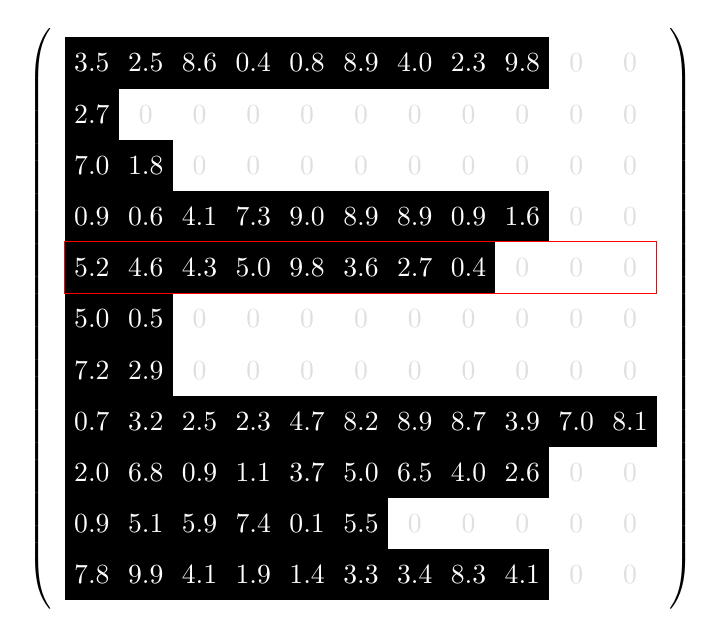
\begin{tikzpicture}[>=latex]
\matrix (A) [matrix of math nodes,
            nodes = {whclsty},
            left delimiter  = (,
            right delimiter = ),
            ampersand replacement=\&,
            anchor=north west] at (0,0)
{
|[nzsty]|3.5 \& |[nzsty]|2.5 \& |[nzsty]|8.6 \& |[nzsty]|0.4 \& |[nzsty]|0.8 \& |[nzsty]|8.9 \& |[nzsty]|4.0 \& |[nzsty]|2.3 \& |[nzsty]|9.8 \& \zecl \& \zecl \\
|[nzsty]|2.7 \& \zecl \& \zecl \& \zecl \& \zecl \& \zecl \& \zecl \& \zecl \& \zecl \& \zecl \& \zecl \\
|[nzsty]|7.0 \& |[nzsty]|1.8 \& \zecl \& \zecl \& \zecl \& \zecl \& \zecl \& \zecl \& \zecl \& \zecl \& \zecl \\
|[nzsty]|0.9 \& |[nzsty]|0.6 \& |[nzsty]|4.1 \& |[nzsty]|7.3 \& |[nzsty]|9.0 \& |[nzsty]|8.9 \& |[nzsty]|8.9 \& |[nzsty]|0.9 \& |[nzsty]|1.6 \& \zecl \& \zecl \\
|[nzsty]|5.2 \& |[nzsty]|4.6 \& |[nzsty]|4.3 \& |[nzsty]|5.0 \& |[nzsty]|9.8 \& |[nzsty]|3.6 \& |[nzsty]|2.7 \& |[nzsty]|0.4 \& \zecl \& \zecl \& \zecl \\
|[nzsty]|5.0 \& |[nzsty]|0.5 \& \zecl \& \zecl \& \zecl \& \zecl \& \zecl \& \zecl \& \zecl \& \zecl \& \zecl \\
|[nzsty]|7.2 \& |[nzsty]|2.9 \& \zecl \& \zecl \& \zecl \& \zecl \& \zecl \& \zecl \& \zecl \& \zecl \& \zecl \\
|[nzsty]|0.7 \& |[nzsty]|3.2 \& |[nzsty]|2.5 \& |[nzsty]|2.3 \& |[nzsty]|4.7 \& |[nzsty]|8.2 \& |[nzsty]|8.9 \& |[nzsty]|8.7 \& |[nzsty]|3.9 \& |[nzsty]|7.0 \& |[nzsty]|8.1 \\
|[nzsty]|2.0 \& |[nzsty]|6.8 \& |[nzsty]|0.9 \& |[nzsty]|1.1 \& |[nzsty]|3.7 \& |[nzsty]|5.0 \& |[nzsty]|6.5 \& |[nzsty]|4.0 \& |[nzsty]|2.6 \& \zecl \& \zecl \\
|[nzsty]|0.9 \& |[nzsty]|5.1 \& |[nzsty]|5.9 \& |[nzsty]|7.4 \& |[nzsty]|0.1 \& |[nzsty]|5.5 \& \zecl \& \zecl \& \zecl \& \zecl \& \zecl \\
|[nzsty]|7.8 \& |[nzsty]|9.9 \& |[nzsty]|4.1 \& |[nzsty]|1.9 \& |[nzsty]|1.4 \& |[nzsty]|3.3 \& |[nzsty]|3.4 \& |[nzsty]|8.3 \& |[nzsty]|4.1 \& \zecl \& \zecl \\
};

\draw[hlsty] (A-5-1.south west) rectangle (A-5-11.north east);
\end{tikzpicture}}
\aftermatrix
\end{minipage}
\scalebox{\formatscale}{%
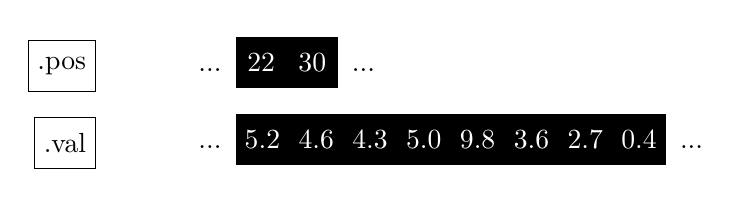
\begin{tikzpicture}[>=latex]
  \matrix (vals) [matrix of math nodes,
              nodes = {whclsty},
              ampersand replacement=\&,
              anchor=north west] at (0,0)
  {
  ... \& |[nzsty]|5.2 \& |[nzsty]|4.6 \& |[nzsty]|4.3 \& |[nzsty]|5.0 \& |[nzsty]|9.8 \& |[nzsty]|3.6 \& |[nzsty]|2.7 \& |[nzsty]|0.4 \& ... \\
  };
  \node [draw, whclsty, left=of vals] {\juliainline{.val}};

  \matrix (pos) [matrix of math nodes,
              nodes = {whclsty},
              ampersand replacement=\&,
              anchor=north west] at (0,1.5 * \myunit)
  {
  ... \& |[nzsty]|22 \& |[nzsty]| 30 \& ... \\
  };
  \node [draw, whclsty, left=of pos] {\juliainline{.pos}};

\end{tikzpicture}%
}
\afterformat
\resizebox{\linewidth}{!}{%
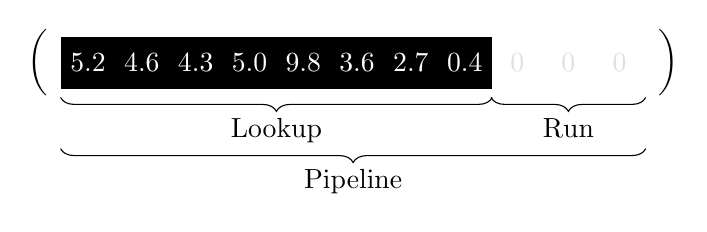
\begin{tikzpicture}[>=latex]
  \matrix (A) [matrix of math nodes,
              nodes = {whclsty},
              left delimiter  = (,
              right delimiter = ),
              ampersand replacement=\&] at (0,0)
  {
  |[nzsty]|5.2 \& |[nzsty]|4.6 \& |[nzsty]|4.3 \& |[nzsty]|5.0 \& |[nzsty]|9.8 \& |[nzsty]|3.6 \& |[nzsty]|2.7 \& |[nzsty]|0.4 \& \zecl \& \zecl \& \zecl \\
  };

  \draw[lpltsty] ([yshift=-0*\myunit]A-1-1.south west) -- ([yshift=-0*\myunit]A-1-8.south east) node[namesty]{Lookup};
  \draw[lpltsty] ([yshift=-0*\myunit]A-1-9.south west) -- ([yshift=-0*\myunit]A-1-11.south east) node[namesty]{Run};
  \draw[lpltsty] ([yshift=-1*\myunit]A-1-1.south west) -- ([yshift=-1*\myunit]A-1-11.south east) node[namesty]{Pipeline};
\end{tikzpicture}%
}  
\begin{juliacode}
Pipeline(
  Phase(
    stride = pos[i+1]-pos[i],
    body = Lookup(
      body(j) = val[pos[i]+j-1])),
  Phase(
    body = Run(0)))
\end{juliacode}
\caption{Ragged}\label{fig:structure:ragged}
\end{subfigure}
\beforematrix


\begin{subfigure}{\linewidth}
\begin{minipage}{\matrixscale\linewidth}
\documentclass{standalone}
\usepackage{tikz}
\usetikzlibrary{matrix,arrows,decorations.pathmorphing,decorations.pathreplacing,calc,positioning}
\usepackage{xcolor}
% all other packages and stuff you need for the picture
\newcommand{\myunit}{0.65 cm}
\newcommand{\myraise}{3pt}
\tikzset{
    lpltsty/.style={decorate, decoration = {brace,mirror,raise=3pt,amplitude=5pt}},
    namesty/.style={pos=0.5,below=7pt},
    scalarsty/.style={draw,fill=white,rectangle,minimum size=\myunit,anchor=center},
    indexsty/.style={fill,fill=white,rectangle,minimum width=\myunit,anchor=center},
    touchsty/.style={fill,fill=red,rectangle,minimum size=\myunit},
    ycsty/.style={fill,fill=yellow,rectangle,minimum size=\myunit},
    brcsty/.style={fill,fill=brown,rectangle,minimum size=\myunit},
    blcsty/.style={fill,fill=cyan!20,rectangle,minimum size=\myunit},
    becsty/.style={fill,fill=beige,rectangle,minimum size=\myunit},
    ocsty/.style={fill,fill=orange,rectangle,minimum size=\myunit},
    whclsty/.style={fill,fill=white,rectangle,minimum size=\myunit},
    zcsty/.style={fill,fill=white,rectangle,minimum size=\myunit,text=zerogray},
    nzsty/.style={fill,fill=black,rectangle,minimum size=\myunit,text=white},
    rcsty/.style={fill,fill=purple,rectangle,minimum size=\myunit},
    pcsty/.style={fill,fill=pink,rectangle,minimum size=\myunit},
    lcsty/.style={fill,fill=blue,rectangle,minimum size=\myunit},
    bcsty/.style={fill,fill=black,rectangle,minimum size=\myunit, text=white},
    hlsty/.style={draw=red},
}


\colorlet{zerogray}{gray!25}
\colorlet{beige}{brown!70}

\newcommand{\ylcl}{|[ycsty]|1}
\newcommand{\recl}{|[rcsty]|2}
\newcommand{\picl}{|[pcsty]|3}
\newcommand{\blcl}{|[blcsty]|1}
\newcommand{\brcl}{|[brcsty]|2}
\newcommand{\becl}{|[becsty]|3}
\newcommand{\orcl}{|[ocsty]|4}
\newcommand{\bkcl}{|[bcsty]|5}
\newcommand{\whcl}{|[whclsty]|0}
\newcommand{\zecl}{|[zcsty]|0}

\newcommand{\formatscale}{0.5}
\newcommand{\matrixscale}{0.69}
\begin{document}

\resizebox{\linewidth}{!}{%
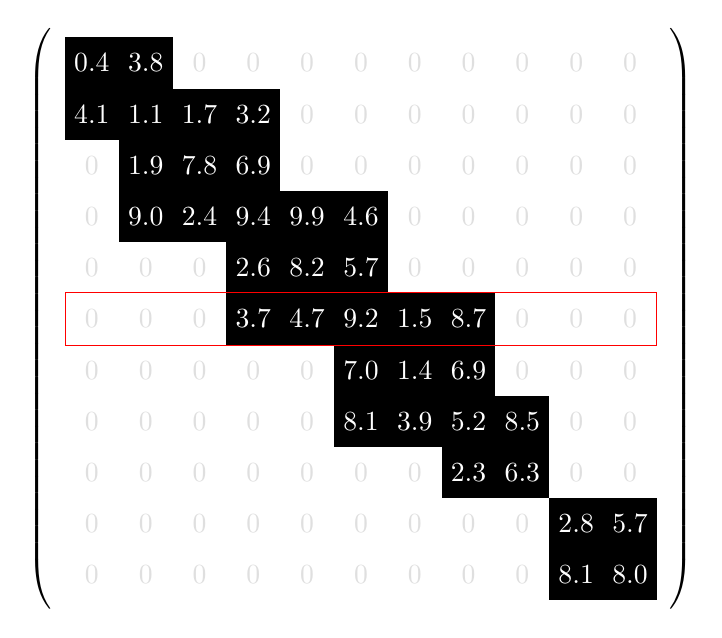
\begin{tikzpicture}[>=latex]
\matrix (A) [matrix of math nodes,
  nodes = {whclsty},
  left delimiter  = (,
  right delimiter = ),
  ampersand replacement=\&] at (0,0)
{
|[nzsty]|0.4 \& |[nzsty]|3.8 \& \zecl \& \zecl \& \zecl \& \zecl \& \zecl \& \zecl \& \zecl \& \zecl \& \zecl \\
|[nzsty]|4.1 \& |[nzsty]|1.1 \& |[nzsty]|1.7 \& |[nzsty]|3.2 \& \zecl \& \zecl \& \zecl \& \zecl \& \zecl \& \zecl \& \zecl \\
\zecl \& |[nzsty]|1.9 \& |[nzsty]|7.8 \& |[nzsty]|6.9 \& \zecl \& \zecl \& \zecl \& \zecl \& \zecl \& \zecl \& \zecl \\
\zecl \& |[nzsty]|9.0 \& |[nzsty]|2.4 \& |[nzsty]|9.4 \& |[nzsty]|9.9 \& |[nzsty]|4.6 \& \zecl \& \zecl \& \zecl \& \zecl \& \zecl \\
\zecl \& \zecl \& \zecl \& |[nzsty]|2.6 \& |[nzsty]|8.2 \& |[nzsty]|5.7 \& \zecl \& \zecl \& \zecl \& \zecl \& \zecl \\
\zecl \& \zecl \& \zecl \& |[nzsty]|3.7 \& |[nzsty]|4.7 \& |[nzsty]|9.2 \& |[nzsty]|1.5 \& |[nzsty]|8.7 \& \zecl \& \zecl \& \zecl \\
\zecl \& \zecl \& \zecl \& \zecl \& \zecl \& |[nzsty]|7.0 \& |[nzsty]|1.4 \& |[nzsty]|6.9 \& \zecl \& \zecl \& \zecl \\
\zecl \& \zecl \& \zecl \& \zecl \& \zecl \& |[nzsty]|8.1 \& |[nzsty]|3.9 \& |[nzsty]|5.2 \& |[nzsty]|8.5 \& \zecl \& \zecl \\
\zecl \& \zecl \& \zecl \& \zecl \& \zecl \& \zecl \& \zecl \& |[nzsty]|2.3 \& |[nzsty]|6.3 \& \zecl \& \zecl \\
\zecl \& \zecl \& \zecl \& \zecl \& \zecl \& \zecl \& \zecl \& \zecl \& \zecl \& |[nzsty]|2.8 \& |[nzsty]|5.7 \\
\zecl \& \zecl \& \zecl \& \zecl  \& \zecl \& \zecl \& \zecl \& \zecl \& \zecl \& |[nzsty]|8.1 \& |[nzsty]|8.0 \\
};

\draw[hlsty] (A-6-1.south west) rectangle (A-6-11.north east);
\end{tikzpicture}}
\end{document}
\aftermatrix
\end{minipage}
\scalebox{\formatscale}{%
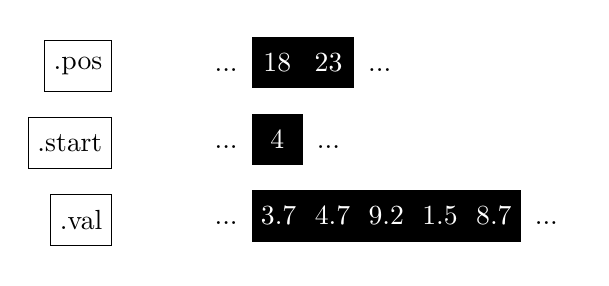
\begin{tikzpicture}[>=latex]
  \matrix (vals) [matrix of math nodes,
              nodes = {whclsty},
              ampersand replacement=\&,
              anchor=north west] at (0,0)
  {
  ... \& |[nzsty]|3.7 \& |[nzsty]|4.7 \& |[nzsty]|9.2 \& |[nzsty]|1.5 \& |[nzsty]|8.7 \& ... \\
  };
  \node [draw, whclsty, left=of vals] {\juliainline{.val}};

  \matrix (start) [matrix of math nodes,
              nodes = {whclsty},
              ampersand replacement=\&,
              anchor=north west] at (0,1.5 * \myunit)
  {
  ... \& |[nzsty]|4 \& ... \\
  };
  \node [draw, whclsty, left=of start] {\juliainline{.start}};

  \matrix (pos) [matrix of math nodes,
              nodes = {whclsty},
              ampersand replacement=\&,
              anchor=north west] at (0,3 * \myunit)
  {
  ... \& |[nzsty]|18 \& |[nzsty]| 23 \& ... \\
  };
  \node [draw, whclsty, left=of pos] {\juliainline{.pos}};

\end{tikzpicture}%
}

\documentclass{standalone}
\usepackage{tikz}
% all other packages and stuff you need for the picture
\newcommand{\myunit}{0.65 cm}
  \newcommand{\myraise}{3pt}
\tikzset{
    lpltsty/.style={decorate, decoration = {brace,mirror,raise=3pt,amplitude=5pt}},
    namesty/.style={pos=0.5,below=7pt},
    scalarsty/.style={draw,fill=white,rectangle,minimum size=\myunit,anchor=center},
    indexsty/.style={fill,fill=white,rectangle,minimum width=\myunit,anchor=center},
    touchsty/.style={fill,fill=red,rectangle,minimum size=\myunit},
    ycsty/.style={fill,fill=yellow,rectangle,minimum size=\myunit},
    brcsty/.style={fill,fill=brown,rectangle,minimum size=\myunit},
    blcsty/.style={fill,fill=cyan!20,rectangle,minimum size=\myunit},
    becsty/.style={fill,fill=beige,rectangle,minimum size=\myunit},
    ocsty/.style={fill,fill=orange,rectangle,minimum size=\myunit},
    whclsty/.style={fill,fill=white,rectangle,minimum size=\myunit},
    zcsty/.style={fill,fill=white,rectangle,minimum size=\myunit,text=zerogray},
    nzsty/.style={fill,fill=black,rectangle,minimum size=\myunit,text=white},
    rcsty/.style={fill,fill=purple,rectangle,minimum size=\myunit},
    pcsty/.style={fill,fill=pink,rectangle,minimum size=\myunit},
    lcsty/.style={fill,fill=blue,rectangle,minimum size=\myunit},
    bcsty/.style={fill,fill=black,rectangle,minimum size=\myunit, text=white},
    hlsty/.style={draw=red},
}
\usepackage{tikz}
\usetikzlibrary{matrix,arrows,decorations.pathmorphing,decorations.pathreplacing,calc,positioning}
\usepackage{xcolor}
\colorlet{zerogray}{gray!25}
\colorlet{beige}{brown!70}

\newcommand{\ylcl}{|[ycsty]|1}
\newcommand{\recl}{|[rcsty]|2}
\newcommand{\picl}{|[pcsty]|3}
\newcommand{\blcl}{|[blcsty]|1}
\newcommand{\brcl}{|[brcsty]|2}
\newcommand{\becl}{|[becsty]|3}
\newcommand{\orcl}{|[ocsty]|4}
\newcommand{\bkcl}{|[bcsty]|5}
\newcommand{\whcl}{|[whclsty]|0}
\newcommand{\zecl}{|[zcsty]|0}

\newcommand{\formatscale}{0.5}
\newcommand{\matrixscale}{0.69}
\newcommand{\aftermatrix}{\vspace{-10pt}}
\newcommand{\afterformat}{\vspace{-5pt}}
\newcommand{\beforematrix}{\vspace{10pt}}

\begin{document}
\begin{tikzpicture}
% your picture code
\end{tikzpicture}
\end{document}
\afterformat
\resizebox{\linewidth}{!}{%
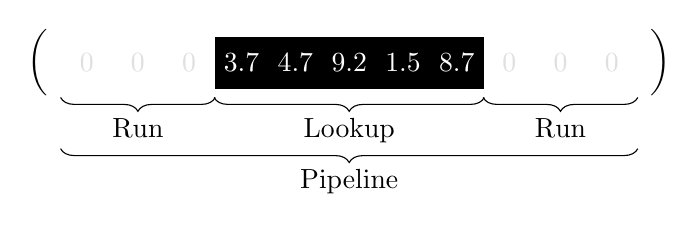
\begin{tikzpicture}[>=latex]
  \matrix (A) [matrix of math nodes,
              nodes = {whclsty},
              left delimiter  = (,
              right delimiter = ),
              ampersand replacement=\&] at (0,0)
  {
  \zecl \& \zecl \& \zecl \& |[nzsty]|3.7 \& |[nzsty]|4.7 \& |[nzsty]|9.2 \& |[nzsty]|1.5 \& |[nzsty]|8.7 \& \zecl \& \zecl \& \zecl \\
  };

  \draw[lpltsty] ([yshift=-0*\myunit]A-1-1.south west) -- ([yshift=-0*\myunit]A-1-3.south east) node[namesty]{Run};
  \draw[lpltsty] ([yshift=-0*\myunit]A-1-4.south west) -- ([yshift=-0*\myunit]A-1-8.south east) node[namesty]{Lookup};
  \draw[lpltsty] ([yshift=-0*\myunit]A-1-9.south west) -- ([yshift=-0*\myunit]A-1-11.south east) node[namesty]{Run};
  \draw[lpltsty] ([yshift=-1*\myunit]A-1-1.south west) -- ([yshift=-1*\myunit]A-1-11.south east) node[namesty]{Pipeline};
\end{tikzpicture}%
}  
\begin{juliacode}
band = pos[i + 1] - pos[i]
offset = pos[i] - start[i]
Pipeline(
  Phase(
    stride = start[i] - 1
    body = Run(0)),
  Phase(
    stride = start[i] + band - 1,
    body = Lookup(
      body(j) = vals[offset + j])),
  Phase(
    body = Run(0)))
\end{juliacode}
\caption{Banded Matrix, Band Format}\label{fig:structure:band}
\end{subfigure}


\end{minipage}\hspace{4pt}%
\begin{minipage}[t]{0.25\linewidth - 3pt}

\begin{subfigure}[t]{\linewidth}
\begin{minipage}[t]{\matrixscale\linewidth}
\documentclass{standalone}
\usepackage{tikz}
\usetikzlibrary{matrix,arrows,decorations.pathmorphing,decorations.pathreplacing,calc,positioning}
\usepackage{xcolor}
% all other packages and stuff you need for the picture
\newcommand{\myunit}{0.65 cm}
\newcommand{\myraise}{3pt}
\tikzset{
    lpltsty/.style={decorate, decoration = {brace,mirror,raise=3pt,amplitude=5pt}},
    namesty/.style={pos=0.5,below=7pt},
    scalarsty/.style={draw,fill=white,rectangle,minimum size=\myunit,anchor=center},
    indexsty/.style={fill,fill=white,rectangle,minimum width=\myunit,anchor=center},
    touchsty/.style={fill,fill=red,rectangle,minimum size=\myunit},
    ycsty/.style={fill,fill=yellow,rectangle,minimum size=\myunit},
    brcsty/.style={fill,fill=brown,rectangle,minimum size=\myunit},
    blcsty/.style={fill,fill=cyan!20,rectangle,minimum size=\myunit},
    becsty/.style={fill,fill=beige,rectangle,minimum size=\myunit},
    ocsty/.style={fill,fill=orange,rectangle,minimum size=\myunit},
    whclsty/.style={fill,fill=white,rectangle,minimum size=\myunit},
    zcsty/.style={fill,fill=white,rectangle,minimum size=\myunit,text=zerogray},
    nzsty/.style={fill,fill=black,rectangle,minimum size=\myunit,text=white},
    rcsty/.style={fill,fill=purple,rectangle,minimum size=\myunit},
    pcsty/.style={fill,fill=pink,rectangle,minimum size=\myunit},
    lcsty/.style={fill,fill=blue,rectangle,minimum size=\myunit},
    bcsty/.style={fill,fill=black,rectangle,minimum size=\myunit, text=white},
    hlsty/.style={draw=red},
}


\colorlet{zerogray}{gray!25}
\colorlet{beige}{brown!70}

\newcommand{\ylcl}{|[ycsty]|1}
\newcommand{\recl}{|[rcsty]|2}
\newcommand{\picl}{|[pcsty]|3}
\newcommand{\blcl}{|[blcsty]|1}
\newcommand{\brcl}{|[brcsty]|2}
\newcommand{\becl}{|[becsty]|3}
\newcommand{\orcl}{|[ocsty]|4}
\newcommand{\bkcl}{|[bcsty]|5}
\newcommand{\whcl}{|[whclsty]|0}
\newcommand{\zecl}{|[zcsty]|0}

\newcommand{\formatscale}{0.5}
\newcommand{\matrixscale}{0.69}
\begin{document}

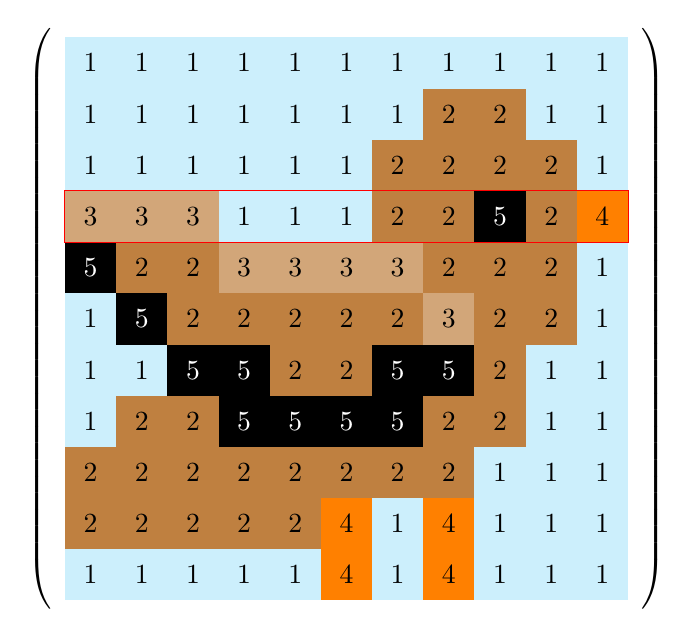
\begin{tikzpicture}[>=latex]
\matrix (A) [matrix of math nodes,
  nodes = {whclsty},
  left delimiter  = (,
  right delimiter = ),
  ampersand replacement=\&] at (0,0)
{
  \blcl \& \blcl \& \blcl \& \blcl \& \blcl \& \blcl \& \blcl \& \blcl \& \blcl \& \blcl \& \blcl\\
  \blcl \& \blcl \& \blcl \& \blcl \& \blcl \& \blcl \& \blcl \& \brcl \& \brcl \& \blcl \& \blcl\\
  \blcl \& \blcl \& \blcl \& \blcl \& \blcl \& \blcl \& \brcl \& \brcl \& \brcl \& \brcl \& \blcl\\
  \becl \& \becl \& \becl \& \blcl \& \blcl \& \blcl \& \brcl \& \brcl \& \bkcl \& \brcl \& \orcl\\
  \bkcl \& \brcl \& \brcl \& \becl \& \becl \& \becl \& \becl \& \brcl \& \brcl \& \brcl \& \blcl\\
  \blcl \& \bkcl \& \brcl \& \brcl \& \brcl \& \brcl \& \brcl \& \becl \& \brcl \& \brcl \& \blcl\\
  \blcl \& \blcl \& \bkcl \& \bkcl \& \brcl \& \brcl \& \bkcl \& \bkcl \& \brcl \& \blcl \& \blcl\\
  \blcl \& \brcl \& \brcl \& \bkcl \& \bkcl \& \bkcl \& \bkcl \& \brcl \& \brcl \& \blcl \& \blcl\\
  \brcl \& \brcl \& \brcl \& \brcl \& \brcl \& \brcl \& \brcl \& \brcl \& \blcl \& \blcl \& \blcl\\
  \brcl \& \brcl \& \brcl \& \brcl \& \brcl \& \orcl \& \blcl \& \orcl \& \blcl \& \blcl \& \blcl\\
  \blcl \& \blcl \& \blcl \& \blcl \& \blcl \& \orcl \& \blcl \& \orcl \& \blcl \& \blcl \& \blcl\\
};

\draw[hlsty] (A-4-1.south west) rectangle (A-4-11.north east);
\end{tikzpicture}
\end{document}
\aftermatrix
\end{minipage}
\scalebox{\formatscale}{%
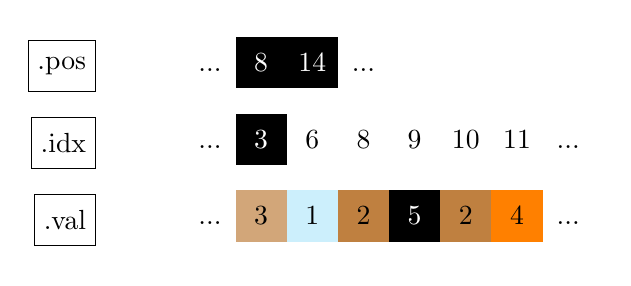
\begin{tikzpicture}[>=latex]
  \matrix (vals) [matrix of math nodes,
              nodes = {whclsty},
              ampersand replacement=\&,
              anchor=north west] at (0,0)
  {
  ... \& \becl \& \blcl \& \& \brcl \& \bkcl \& \brcl \& \orcl \& ...\\
  };
  \node [draw, whclsty, left=of vals] {\juliainline{.val}};

  \matrix (idx) [matrix of math nodes,
              nodes = {whclsty},
              ampersand replacement=\&,
              anchor=north west] at (0,1.5 * \myunit)
  {
  ... \& |[nzsty]|3 \& 6 \& 8 \& 9 \& 10 \& 11 \& ... \\
  };
  \node [draw, whclsty, left=of idx] {\juliainline{.idx}};

  \matrix (pos) [matrix of math nodes,
              nodes = {whclsty},
              ampersand replacement=\&,
              anchor=north west] at (0,3 * \myunit)
  {
  ... \& |[nzsty]|8 \& |[nzsty]| 14 \& ... \\
  };
  \node [draw, whclsty, left=of pos] {\juliainline{.pos}};

\end{tikzpicture}%
}
\afterformat
\resizebox{\linewidth}{!}{%
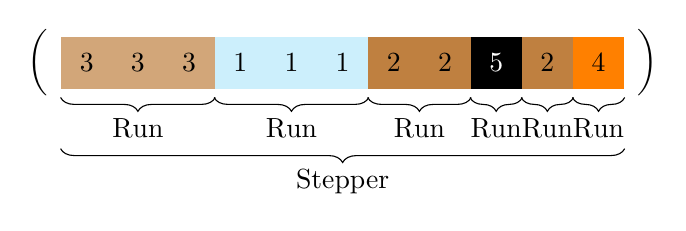
\begin{tikzpicture}[>=latex]
  \matrix (A) [matrix of math nodes,
              nodes = {whclsty},
              left delimiter  = (,
              right delimiter = ),
              ampersand replacement=\&] at (0,0)
  {
  \becl \& \becl \& \becl \& \blcl \& \blcl \& \blcl \& \brcl \& \brcl \& \bkcl \& \brcl \& \orcl\\
  };

  \draw[lpltsty] ([yshift=-0*\myunit]A-1-1.south west) -- ([yshift=-0*\myunit]A-1-3.south east) node[namesty]{Run};
  \draw[lpltsty] ([yshift=-0*\myunit]A-1-4.south west) -- ([yshift=-0*\myunit]A-1-6.south east) node[namesty]{Run};
  \draw[lpltsty] ([yshift=-0*\myunit]A-1-7.south west) -- ([yshift=-0*\myunit]A-1-8.south east) node[namesty]{Run};
  \draw[lpltsty] ([yshift=-0*\myunit]A-1-9.south west) -- ([yshift=-0*\myunit]A-1-9.south east) node[namesty]{Run};
  \draw[lpltsty] ([yshift=-0*\myunit]A-1-10.south west) -- ([yshift=-0*\myunit]A-1-10.south east) node[namesty]{Run};
  \draw[lpltsty] ([yshift=-0*\myunit]A-1-11.south west) -- ([yshift=-0*\myunit]A-1-11.south east) node[namesty]{Run};
  \draw[lpltsty] ([yshift=-1*\myunit]A-1-1.south west) -- ([yshift=-1*\myunit]A-1-11.south east) node[namesty]{Stepper};
\end{tikzpicture}%
} 
\begin{juliacode}
p = pos[i]
Stepper(
  seek(j) = (p = search(idx, j)),
  stride = idx[p],
  body = Run(
    body = val[p]),
  next = p += 1)
\end{juliacode}
\caption{Image with repeated values. Run-Length Format.}\label{fig:structure:birb-rle}
\end{subfigure}
\beforematrix

\begin{subfigure}{\linewidth}
\begin{minipage}{\matrixscale\linewidth}
\documentclass{standalone}
\usepackage{tikz}
\usetikzlibrary{matrix,arrows,decorations.pathmorphing,decorations.pathreplacing,calc,positioning}
\usepackage{xcolor}
% all other packages and stuff you need for the picture
\newcommand{\myunit}{0.65 cm}
\newcommand{\myraise}{3pt}
\tikzset{
    lpltsty/.style={decorate, decoration = {brace,mirror,raise=3pt,amplitude=5pt}},
    namesty/.style={pos=0.5,below=7pt},
    scalarsty/.style={draw,fill=white,rectangle,minimum size=\myunit,anchor=center},
    indexsty/.style={fill,fill=white,rectangle,minimum width=\myunit,anchor=center},
    touchsty/.style={fill,fill=red,rectangle,minimum size=\myunit},
    ycsty/.style={fill,fill=yellow,rectangle,minimum size=\myunit},
    brcsty/.style={fill,fill=brown,rectangle,minimum size=\myunit},
    blcsty/.style={fill,fill=cyan!20,rectangle,minimum size=\myunit},
    becsty/.style={fill,fill=beige,rectangle,minimum size=\myunit},
    ocsty/.style={fill,fill=orange,rectangle,minimum size=\myunit},
    whclsty/.style={fill,fill=white,rectangle,minimum size=\myunit},
    zcsty/.style={fill,fill=white,rectangle,minimum size=\myunit,text=zerogray},
    nzsty/.style={fill,fill=black,rectangle,minimum size=\myunit,text=white},
    rcsty/.style={fill,fill=purple,rectangle,minimum size=\myunit},
    pcsty/.style={fill,fill=pink,rectangle,minimum size=\myunit},
    lcsty/.style={fill,fill=blue,rectangle,minimum size=\myunit},
    bcsty/.style={fill,fill=black,rectangle,minimum size=\myunit, text=white},
    hlsty/.style={draw=red},
}


\colorlet{zerogray}{gray!25}
\colorlet{beige}{brown!70}

\newcommand{\ylcl}{|[ycsty]|1}
\newcommand{\recl}{|[rcsty]|2}
\newcommand{\picl}{|[pcsty]|3}
\newcommand{\blcl}{|[blcsty]|1}
\newcommand{\brcl}{|[brcsty]|2}
\newcommand{\becl}{|[becsty]|3}
\newcommand{\orcl}{|[ocsty]|4}
\newcommand{\bkcl}{|[bcsty]|5}
\newcommand{\whcl}{|[whclsty]|0}
\newcommand{\zecl}{|[zcsty]|0}

\newcommand{\formatscale}{0.5}
\newcommand{\matrixscale}{0.69}
\begin{document}

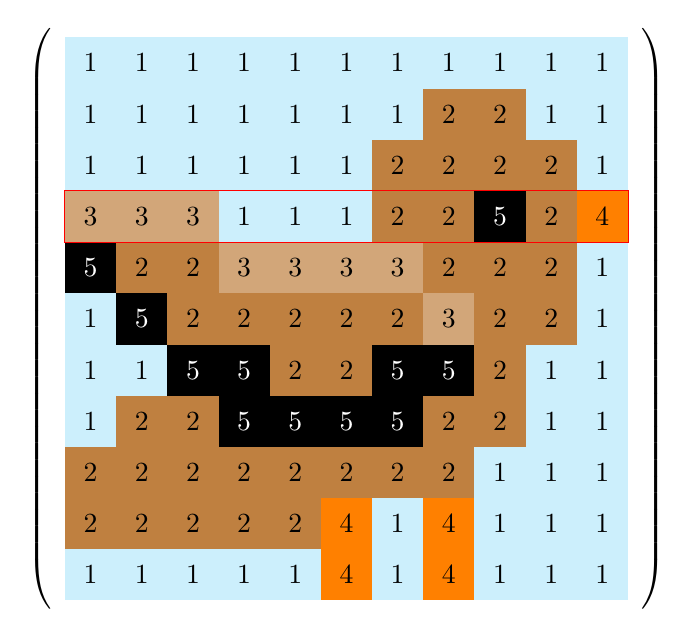
\begin{tikzpicture}[>=latex]
\matrix (A) [matrix of math nodes,
  nodes = {whclsty},
  left delimiter  = (,
  right delimiter = ),
  ampersand replacement=\&] at (0,0)
{
  \blcl \& \blcl \& \blcl \& \blcl \& \blcl \& \blcl \& \blcl \& \blcl \& \blcl \& \blcl \& \blcl\\
  \blcl \& \blcl \& \blcl \& \blcl \& \blcl \& \blcl \& \blcl \& \brcl \& \brcl \& \blcl \& \blcl\\
  \blcl \& \blcl \& \blcl \& \blcl \& \blcl \& \blcl \& \brcl \& \brcl \& \brcl \& \brcl \& \blcl\\
  \becl \& \becl \& \becl \& \blcl \& \blcl \& \blcl \& \brcl \& \brcl \& \bkcl \& \brcl \& \orcl\\
  \bkcl \& \brcl \& \brcl \& \becl \& \becl \& \becl \& \becl \& \brcl \& \brcl \& \brcl \& \blcl\\
  \blcl \& \bkcl \& \brcl \& \brcl \& \brcl \& \brcl \& \brcl \& \becl \& \brcl \& \brcl \& \blcl\\
  \blcl \& \blcl \& \bkcl \& \bkcl \& \brcl \& \brcl \& \bkcl \& \bkcl \& \brcl \& \blcl \& \blcl\\
  \blcl \& \brcl \& \brcl \& \bkcl \& \bkcl \& \bkcl \& \bkcl \& \brcl \& \brcl \& \blcl \& \blcl\\
  \brcl \& \brcl \& \brcl \& \brcl \& \brcl \& \brcl \& \brcl \& \brcl \& \blcl \& \blcl \& \blcl\\
  \brcl \& \brcl \& \brcl \& \brcl \& \brcl \& \orcl \& \blcl \& \orcl \& \blcl \& \blcl \& \blcl\\
  \blcl \& \blcl \& \blcl \& \blcl \& \blcl \& \orcl \& \blcl \& \orcl \& \blcl \& \blcl \& \blcl\\
};

\draw[hlsty] (A-4-1.south west) rectangle (A-4-11.north east);
\end{tikzpicture}
\end{document}
\aftermatrix
\end{minipage}
\scalebox{\formatscale}{%
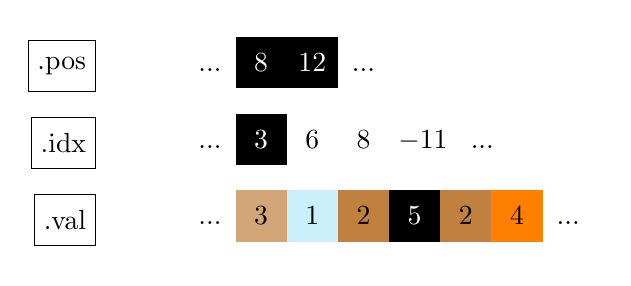
\begin{tikzpicture}[>=latex]
  \matrix (vals) [matrix of math nodes,
              nodes = {whclsty},
              ampersand replacement=\&,
              anchor=north west] at (0,0)
  {
  ... \& \becl \& \blcl \& \& \brcl \& \bkcl \& \brcl \& \orcl \& ...\\
  };
  \node [draw, whclsty, left=of vals] {\juliainline{.val}};

  \matrix (idx) [matrix of math nodes,
              nodes = {whclsty},
              ampersand replacement=\&,
              anchor=north west] at (0,1.5 * \myunit)
  {
  ... \& |[nzsty]|3 \& 6 \& 8 \& -11 \& ... \\
  };
  \node [draw, whclsty, left=of idx] {\juliainline{.idx}};

  \matrix (pos) [matrix of math nodes,
              nodes = {whclsty},
              ampersand replacement=\&,
              anchor=north west] at (0,3 * \myunit)
  {
  ... \& |[nzsty]|8 \& |[nzsty]| 12 \& ... \\
  };
  \node [draw, whclsty, left=of pos] {\juliainline{.pos}};

\end{tikzpicture}%
}
\afterformat
\resizebox{\linewidth}{!}{%
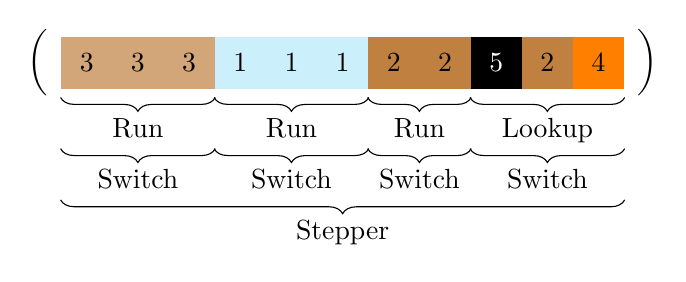
\begin{tikzpicture}[>=latex]
  \matrix (A) [matrix of math nodes,
              nodes = {whclsty},
              left delimiter  = (,
              right delimiter = ),
              ampersand replacement=\&] at (0,0)
  {
  \becl \& \becl \& \becl \& \blcl \& \blcl \& \blcl \& \brcl \& \brcl \& \bkcl \& \brcl \& \orcl\\
  };

  \draw[lpltsty] ([yshift=-0*\myunit]A-1-1.south west) -- ([yshift=-0*\myunit]A-1-3.south east) node[namesty]{Run};
  \draw[lpltsty] ([yshift=-0*\myunit]A-1-4.south west) -- ([yshift=-0*\myunit]A-1-6.south east) node[namesty]{Run};
  \draw[lpltsty] ([yshift=-0*\myunit]A-1-7.south west) -- ([yshift=-0*\myunit]A-1-8.south east) node[namesty]{Run};
  \draw[lpltsty] ([yshift=-0*\myunit]A-1-9.south west) -- ([yshift=-0*\myunit]A-1-11.south east) node[namesty]{Lookup};
  \draw[lpltsty] ([yshift=-1*\myunit]A-1-1.south west) -- ([yshift=-1*\myunit]A-1-3.south east) node[namesty]{Switch};
  \draw[lpltsty] ([yshift=-1*\myunit]A-1-4.south west) -- ([yshift=-1*\myunit]A-1-6.south east) node[namesty]{Switch};
  \draw[lpltsty] ([yshift=-1*\myunit]A-1-7.south west) -- ([yshift=-1*\myunit]A-1-8.south east) node[namesty]{Switch};
  \draw[lpltsty] ([yshift=-1*\myunit]A-1-9.south west) -- ([yshift=-1*\myunit]A-1-11.south east) node[namesty]{Switch};
  \draw[lpltsty] ([yshift=-2*\myunit]A-1-1.south west) -- ([yshift=-2*\myunit]A-1-11.south east) node[namesty]{Stepper};
\end{tikzpicture}%
} 
\begin{juliacode}
s = 0
p = pos[i]
Stepper(
  seek(j) = (
    p = search(abs(idx), j)),
  stride = idx[p],
  body = Switch(
    Case(
      cond = idx[p] > 0,
      body = Run(
        body = vals[p]))
    Case(
      body = Lookup(
        body(j) = vals[p + j - s])))
  next = s = abs(idx[p]); p += 1;)
\end{juliacode}
\caption{Image with repeated values. PackBITS Format.}\label{fig:structure:birb-rlep}
\end{subfigure}

\end{minipage}

\caption{A variety of example structures, corresponding level formats, and
protocols, followed by their corresponding looplet nest unfurling code. Matrices
are row major, and outer levels are dense. The row under consideration is
highlighted in red.}\label{fig:structure}
\end{figure*}